\subsection{Exercise 1}
\subsubsection{Bays29}
\subsubsection*{Base case}
\begin{figure}[H]
    \centering
    \begin{subfigure}[t]{0.5\textwidth}
        \centering
        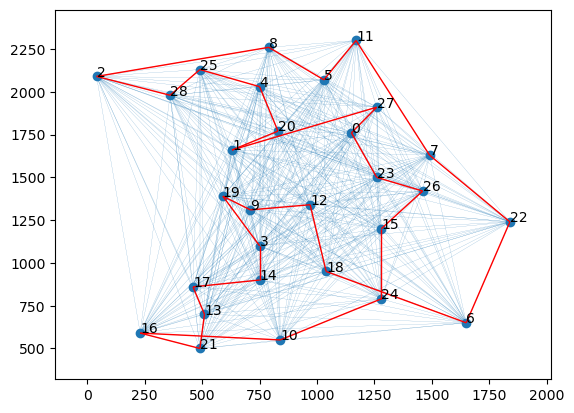
\includegraphics[width=\linewidth]{images/lab7/tsp_base_aco.png}
        \caption{aco solution (distance 2454)}
    \end{subfigure}%
    \begin{subfigure}[t]{0.5\textwidth}
        \centering
        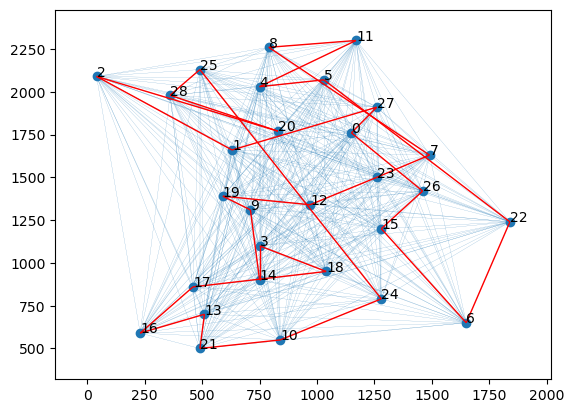
\includegraphics[width=\linewidth]{images/lab7/tsp_base_ea.png}
        \caption{ea solution (distance 3186)}
    \end{subfigure}
    \caption{Optimal distance for bays29=2020}
\end{figure}
\begin{figure}[H]
    \centering
    \begin{subfigure}[t]{0.5\textwidth}
        \centering
        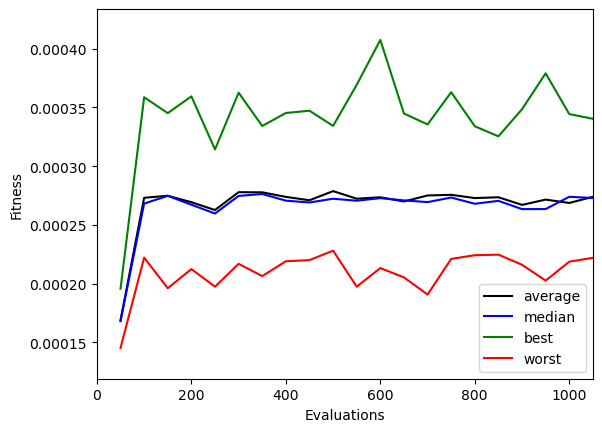
\includegraphics[width=\linewidth]{images/lab7/tsp_base_fitness_aco.png}
        \caption{aco fitness}
    \end{subfigure}%
    \begin{subfigure}[t]{0.5\textwidth}
        \centering
        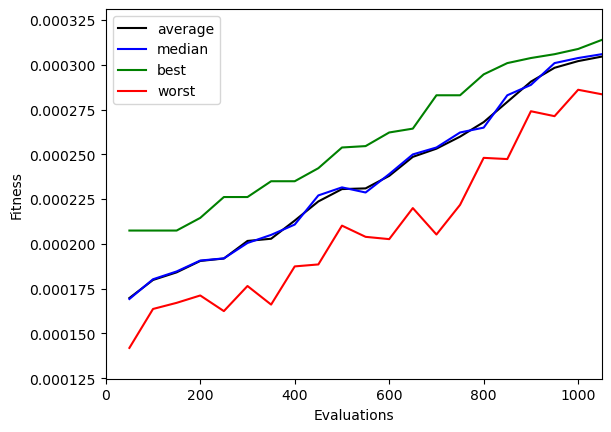
\includegraphics[width=\linewidth]{images/lab7/tsp_base_fitness_ea.png}
        \caption{ea fitness}
    \end{subfigure}
\end{figure}
\begin{comment}
pop\_size = 50
max\_generations = 20
seed = 41
prng = Random(seed)
display = True
# ACS specific parameters
evaporation\_rate = 0.1
learning\_rate = 0.1
# EA specific parameters
tournament\_size = 5
num\_elites = 1
Distance: 2454.0 - Best Solution: [9, 19, 3, 14, 17, 13, 21, 16, 10, 24, 15, 26, 23, 0, 27, 1, 20, 4, 25, 28, 2, 8, 5, 11, 7, 22, 6, 18, 12]
Distance : 3185.9999999999995 - Best Solution EA: [11, 8, 7, 23, 12, 19, 9, 14, 3, 18, 17, 16, 13, 21, 10, 24, 25, 28, 20, 2, 1, 27, 0, 26, 15, 6, 22, 5, 4]
\end{comment}



\subsubsection*{100 generations}
with lots of generations (e.g. 100) ea continues to improve surpassing aco which stay at the same fitness value (we can see this in the fitness graphs
\begin{figure}[H]
    \centering
    \begin{subfigure}[t]{0.5\textwidth}
        \centering
        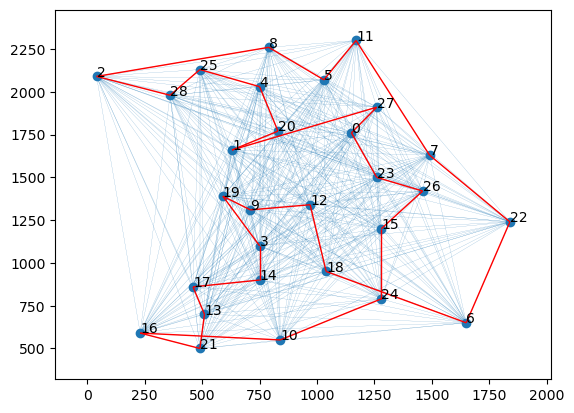
\includegraphics[width=\linewidth]{images/lab7/tsp_100gen_aco.png}
        \caption{aco solution (distance 2454)}
    \end{subfigure}%
    \begin{subfigure}[t]{0.5\textwidth}
        \centering
        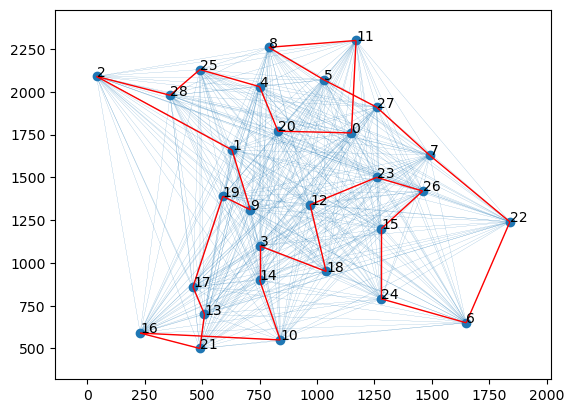
\includegraphics[width=\linewidth]{images/lab7/tsp_100gen_ea.png}
        \caption{ea solution (distance 2361)}
    \end{subfigure}
    \caption{Optimal distance for bays29=2020}
\end{figure}
\begin{figure}[H]
    \centering
    \begin{subfigure}[t]{0.5\textwidth}
        \centering
        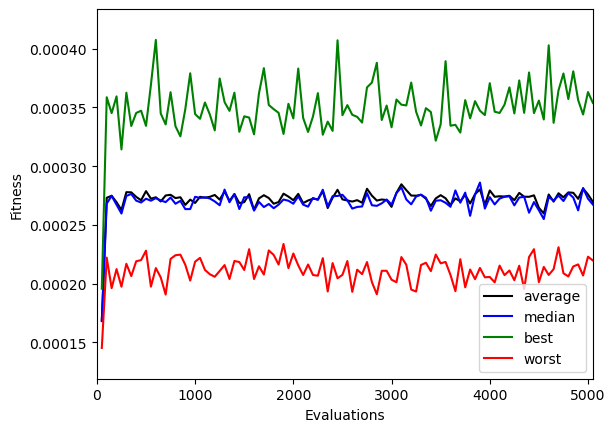
\includegraphics[width=\linewidth]{images/lab7/tsp_100gen_fitness_aco.png}
        \caption{aco fitness}
    \end{subfigure}%
    \begin{subfigure}[t]{0.5\textwidth}
        \centering
        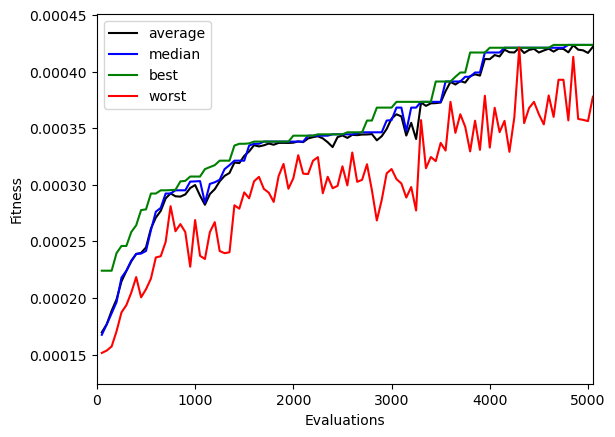
\includegraphics[width=\linewidth]{images/lab7/tsp_100gen_fitness_ea.png}
        \caption{ea fitness}
    \end{subfigure}
\end{figure}
\begin{comment}
 Distance: 2454.0 - Best Solution: [9, 19, 3, 14, 17, 13, 21, 16, 10, 24, 15, 26, 23, 0, 27, 1, 20, 4, 25, 28, 2, 8, 5, 11, 7, 22, 6, 18, 12]
Distance : 2361.0 - Best Solution EA: [28, 25, 4, 20, 0, 11, 8, 5, 27, 7, 22, 6, 24, 15, 26, 23, 12, 18, 3, 14, 10, 16, 21, 13, 17, 19, 9, 1, 2]   
\end{comment}

On the easiest instance of the problem (p01) aco find the optimal path with as little as 10 generation while ea takes at least 75 

\subsubsection{Attr48}
\subsection{Exercise 2}

\subsection{Exercise 3}

\subsection{General questions}